La luce di scintillazione prodotta in un mezzo dal passaggio di una radiazione può essere raccolta da opportuni fotosensori per produrre un segnale elettrico e dare informazioni sulla radiazione originaria. I fotosensori che devono essere accoppiati a uno scintillatore devono essere estremamente sensibili, quindi in grado di produrre un segnale elettrico anche quando vengono colpiti da pochi fotoni. Addirittura certe volte si parla di rivelatori a singolo fotone, quindi anche il singolo fotone può dar luogo a un segnale elettrico rivelabile. In questo capitolo andremo a vedere diverse tipologie di fotosensori, quali i fotomoltiplicatori ma anche rivelatori di più recente produzione come i diodi a valanga e i fotomoltiplicatori realizzati in silicio.

\section{Fotomoltiplicatori}

La prima tipologia di fotosensori che studieremo sono i fotomoltiplicatori.

\subsection{Schema di funzionamento}

Osserviamo come funziona un fotomoltiplicatore:

\begin{figure}[H]
   \centering
   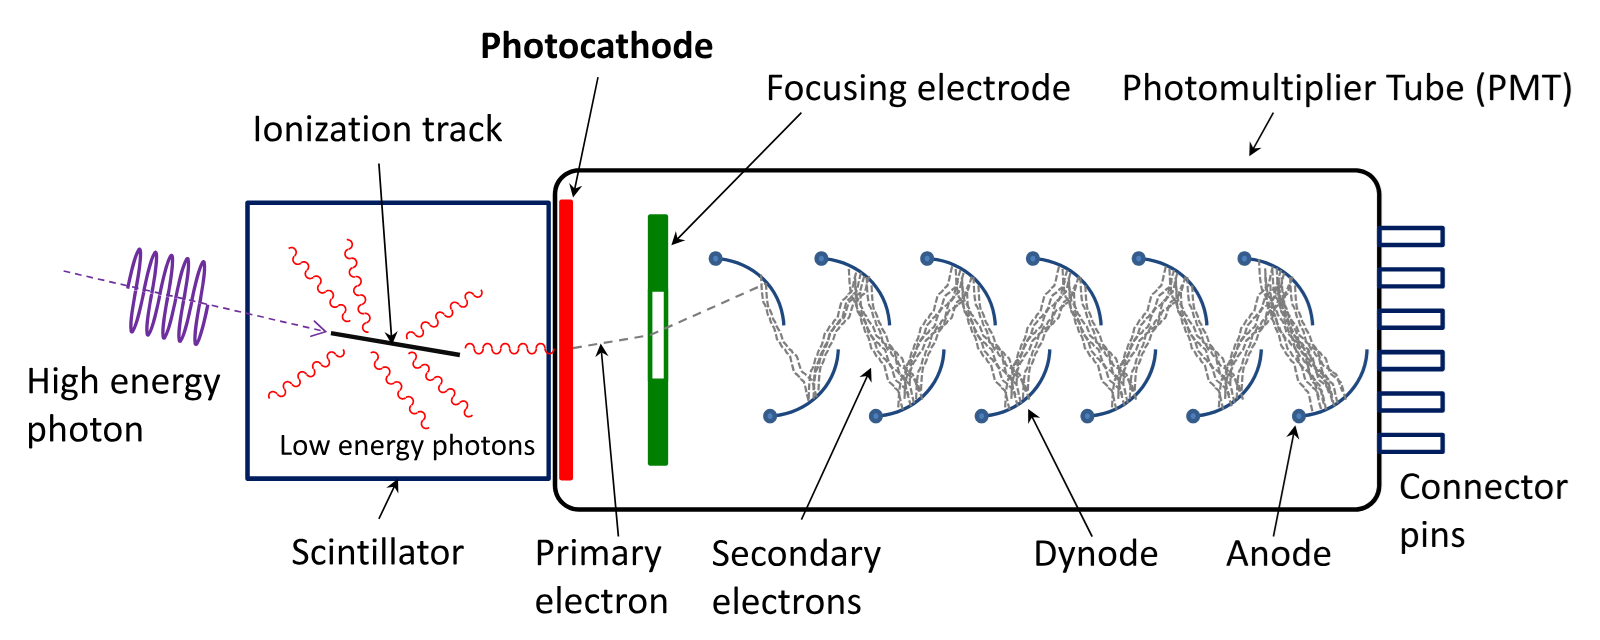
\includegraphics[width=0.8\textwidth]{immagini/fotomoltiplicatore.png}
\end{figure}

Quando arriva una radiazione che interagisce con lo scintillatore in un punto, viene emessa della luce e i fotoni, o attraverso delle riflessioni multiple o perché vengono emessi con la direzione giusta, arrivano alla finestra di ingresso del fotomoltiplicatore che prende il nome di fotocatodo, il quale non è altro che una superficie tipicamente vetrosa che viene rivestita di un materiale con un basso potenziale di estrazione in cui pertanto può facilmente avvenire effetto fotoelettrico, In questo modo, un fotone che incide darà luogo ad effetto fotoelettrico e verrà emesso un elettrone. Quest'ultimo viene guidato verso una zona dove sono presenti degli elettrodi che prendono il nome di dinodi. \E chiaro che l'elettrone viene guidato attraverso un campo elettrico, quindi questi dinodi vengono posizionati ad un potenziale via via crescente, cioè ogni dinodo ha un potenziale maggiore rispetto al precedente, in maniera tale che gli elettroni vengano guidati attraverso questa catena di dinodi.

L'elettrone che viene generato per effetto fotoelettrico, non appena incide sul primo dinodo, permette l'emissione di un certo numero di elettroni, in quanto viene ceduta dell'energia che serve ad estrarre altri elettroni dal primo dinodo; a questo punto tali elettroni vengono accelerati verso il secondo dinodo e ognuno di questi elettroni darà luogo, allo stesso modo, ad altri elettroni. Parliamo quindi di un meccanismo di moltiplicazione, in quanto per ogni dinodo un elettrone incidente può estrarre un certo numero di elettroni.

Tale processo avviene lungo tutta la struttura, quindi man mano il numero di elettroni emessi che viaggia attraverso la catena di dinodi aumenta attraverso una legge di potenza fino a quando arriva all'ultimo dinodo, che non è altro che l'anodo, da cui viene poi prelevato il segnale il quale è un segnale in carica, cioè una corrente, per cui si utilizza una resistenza in modo da produrre un segnale in tensione che è quello che poi adoperiamo e che possiamo visualizzare all'oscilloscopio. Si tratta quindi di un segnale che in linea di principio dovrebbe essere proporzionale al numero di elettroni che sono stati generati da questo fotomoltiplicatore e questo numero di elettroni dipende da quanti fotoni hanno inciso sul fotomoltiplicatore, quindi da quanti fotoni sono stati prodotti durante il processo di scintillazione. In altre parole, si tratta di una catena che permette di mantenere una certa proporzionalità e quindi di avere in uscita un segnale che dà indicazioni sull'energia depositata all'interno dello scintillatore.

A causa di tale schema di funzionamento, il fotomoltiplicatore è un oggetto abbastanza esteso, in quanto dobbiamo avere una catena di dinodi che presenta delle geometrie particolari tali da poter guidare gli elettroni attraverso i dinodi ed inoltre questi devono avere delle forme caratteristiche. Ecco perché si chiama fotomoltiplicatore, perché non solo è un rivelatore di fotoni ma in più è un moltiplicatore, quindi da un singolo elettrone che corrisponde alla rivelazione di un fotone si produce una cascata di elettroni verso l'anodo con un certo fattore di moltiplicazione.

\subsection{Fotocatodo}
Guardiamo un po' più nel dettaglio i diversi componenti del fotomoltiplicatore, partendo dal fotocatodo.

Il fotocatodo rappresenta sostanzialmente la finestra di ingresso al fotomoltiplicatore, quindi è la zona dove devono incidere i fotoni di scintillazione. Normalmente è realizzato su un materiale vetroso\footnote{Il motivo è che così si assicura un indice di rifrazione simile a quello dello scintillatore o delle eventuali guide di luce che si utilizzano per accoppiare lo scintillatore col fotosensore, in maniera tale da evitare fenomeni di rifrazione.} che viene rivestito di un materiale caratterizzato da un un basso lavoro di estrazione. Normalmente vengono utilizzati dei materiali semiconduttori per il semplice fatto che gli elettroni che vengono emessi per effetto fotoelettrico riescono più facilmente a lasciare il fotocatodo e a fuoriuscire. Come sappiamo, l'energia cinetica con cui l'elettrone fuoriesce dipende dall'energia del fotone incidente e dal potenziale di estrazione, essendo data dalla differenza tra queste: poiché i fotoni di scintillazione, ricadendo nell'ultravioletto, hanno energie di circa 3 eV mentre i materiali che si adoperano hanno un potenziale di circa $1.5-2$ eV, l'elettrone che viene emesso ha un'energia abbastanza bassa, di pochi elettronVolt.

Bisogna inoltre ricordare che, essendo un materiale con così basso lavoro di estrazione, potrebbe verificarsi anche un'emissione spontanea per effetto termico. Ad esempio a temperatura ambiente gli elettroni hanno un'energia media di $0,025$ eV, quindi alcuni elettroni potrebbero effettivamente essere emessi per effetto termico. Siccome noi non avvertiamo alcuna differenza tra l'elettrone che viene emesso perché ha inciso un fotone e l'elettrone che viene emesso per effetto termico in quanto entrambi daranno luogo a tutti i processi che abbiamo appena visto, ciò rappresenta un problema perché rappresentano una fonte di rumore che si va a sommare al reale segnale fisico dovuto alla rivelazione di fotoni di scintillazione. Una soluzione banale a tale problema è quella di operare a temperature più basse per ridurre la probabilità di emissione di elettroni per effetto termico.

Come abbiamo detto, l'effetto termico non è del tutto trascurabile. Infatti a temperatura ambiente gli elettroni hanno un'energia media di $0.025$ eV, dunque una certa frazione di elettroni può avere un'energia superiore a questo valore di energia media che risulta sufficiente quindi per poter sfuggire dal materiale. In generale, a temperatura ambiente la frequenza di emissione, cioè il numero di elettroni che vengono emessi al secondo, nei metalli corrisponde a circa 100 elettroni al secondo per ogni metro quadro mentre nei materiali semiconduttori arriva fino a $10^6-10^8$ elettroni al secondo per metro quadro. Capiamo quindi che tale processo non è per niente trascurabile e l'effetto di questa emissione provoca quindi una corrente di elettroni che prende il nome di dark current, perché è una corrente che è sempre presente anche quando non incide luce sul fotosensore, quindi in condizioni di oscurità e purtroppo questo è uno dei parametri di cui si deve tener conto in un fotomoltiplicatore perché rappresenta qualcosa che si somma al segnale.

Un altro aspetto che si deve tenere in conto quando si sceglie il fotocatodo riguarda l'efficienza di rivelazione. Finora infatti abbiamo schematizzato il processo dicendo che la radiazione incide e produce effetto fotoelettrico, ma in realtà la probabilità con cui avviene questo effetto dipende dalla lunghezza d'onda della radiazione incidente. Possiamo quindi andare a definire, in base al tipo di materiale adoperato, quanto vale la quantum efficiency cioè l'efficienza quantica, che rappresenta il numero di fotoelettroni emessi sul numero di fotoni incidenti:
\begin{equation*}
   \text{Quantum Efficiency }(QE)
   =\frac{\text{n° fotoelettroni emessi}}{\text{n° fotoni incidenti}}
\end{equation*}
Per fare un esempio, se incidessero 100 fotoni di scintillazione e in corrispondenza ad ogni fotone di scintillazione ottenessimo un fotoelettrone, allora l'efficienza sarebbe del 100\%. \E chiaro che nella realtà non abbiamo efficienze così elevate: tipicamente ci aggiriamo intorno al $20-30\%$, quindi in media $20-30$ fotoni su 100 riescono a produrre effetto fotoelettrico.

Vediamo adesso le risposte in funzione della lunghezza d'onda per alcuni materiali utilizzati per i fotocatodi:
\begin{figure}[H]
   \centering
   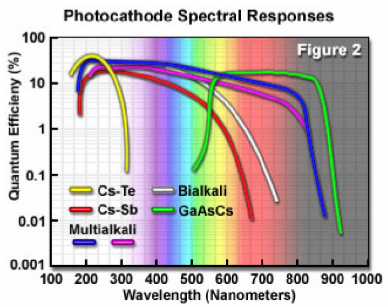
\includegraphics[width=0.65\textwidth]{immagini/efficienza_quantica.png}
\end{figure}
Vediamo come la quantum efficiency è fortemente dipendente dalla lunghezza d'onda, ad esempio ci sono fotocatodi che sono particolarmente ottimizzati per lavorare nel profondo UV e altri invece che lavorano a lunghezza d'onda più elevate. La scelta del fotocatodo dipende dunque fortemente dallo scintillatore che adoperiamo e dallo spettro di emissione di questo, quindi bisogna cercare di far corrispondere queste due finestre di lavoro, cioè l'emissione dello scintillatore e l'assorbimento del fotocatodo.

\subsection{Elettrodi di focalizzazione}
Una volta che sono stati emessi questi elettroni, dobbiamo cercare di convogliarli verso il primo dinodo.

\vspace{-0.3cm}

\begin{minipage}{0.39\textwidth}
   \begin{figure}[H]
      \centering
      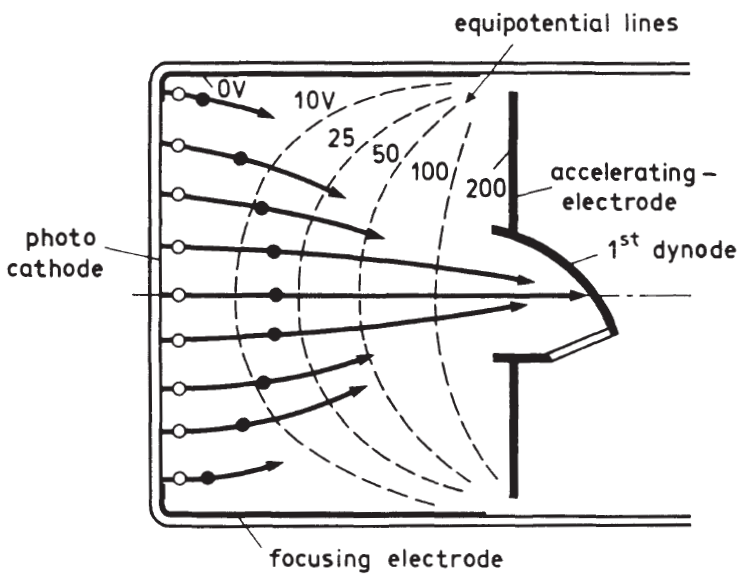
\includegraphics[width=\textwidth]{immagini/elettrodo_di_focalizzazione.png}
   \end{figure}
\end{minipage}
\begin{minipage}{0.6\textwidth}
   \vspace{0.8cm}Come vediamo dalla figura, i fotoni incidono su tutta la superficie del fotocatodo, quindi gli elettroni possono essere emessi da diversi punti e con diverse direzioni, inoltre possono avere energie leggermente diverse. Vogliamo quindi che la raccolta sia efficiente, cioè vorremmo che tutti gli elettroni raggiungessero il primo dinodo indipendentemente dalla loro energia e dal punto in cui sono emessi.
\end{minipage}

\vspace{0.4cm}Per fare questo li dobbiamo in qualche modo guidare. Ecco perché questa prima regione può presentare anche degli elettrodi di focalizzazione, i quali sono degli elettrodi che hanno il compito di accelerare gli elettroni mediante campi elettrici (e alcune volte anche campi magnetici) e fare loro seguire determinati percorsi in base al punto in cui sono emessi, in modo da convogliarli verso il primo dinodo. Il motivo è che, al di là di una questione di efficienza cioè al di là del cercare di convogliare tutti gli elettroni, c'è un problema anche di timing perché gli elettroni che vengono emessi nelle regioni più periferiche devono necessariamente percorrere uno spazio maggiore per arrivare al primo dinodo, e a causa di ciò si corre il rischio di avere degli elettroni che arrivano dopo, il che comporterebbe una indeterminazione dal punto di vista temporale che è ovviamente qualcosa da evitare quando vogliamo adoperare uno scintillatore e un fotomoltiplicatore per misure di timing. 

\subsection{Emissione secondaria e processo di moltiplicazione}
A questo punto cerchiamo di capire cosa avviene nei vari dinodi. L'abbiamo accennato prima: ogni elettrone è in grado di emettere ulteriori elettroni, i quali vengono emessi con energia molto basse di circa 1 eV e ogni dinodo è posto a una differenza di potenziale di circa 100 V rispetto al precedente, in maniera tale che gli elettroni vengano guidati verso i dinodi successivi.

Poiché l'elettrone viene accelerato e quindi acquisisce una certa energia, quando incide sul primo dinodo può estrarre da questo un certo numero di elettroni; in particolare ne estrae all'incirca una trentina, quindi ogni volta che incide un elettrone vengono emessi per effetti secondari una trentina di elettroni, i quali devono essere accelerati verso il secondo dinodo. Tuttavia non tutti questi elettroni riescono ad arrivare al secondo dinodo a causa dell'efficienza di raccolta, per cui solamente una frazione di questi elettroni riesce ad arrivare al secondo dinodo. Tipicamente questa frazione è all'incirca di 5 elettroni su 30. Considerata questa efficienza, possiamo dire che il primo elettrone dà luogo in media a 5 elettroni in grado di arrivare al secondo dinodo. Questo numero, che abbiamo detto aggirarsi normalmente intorno a 5, lo chiamiamo $\delta$ e ora vedremo che importanza ha in termini di formazione del segnale. Dobbiamo quindi immaginare che arrivano $\delta$ elettroni sul secondo dinodo e ognuno di questi darà luogo nel terzo dinodo ad altri $\delta$ elettroni e così via. \E allora evidente che ci sia un meccanismo di moltiplicazione (rappresentato nello schema di funzionamento dalle linee che diventano via via sempre più numerose man mano che si passa da un dinodo al successivo), per cui ci chiediamo quanto valga il \textit{fattore di guadagno}, cioè quanto valga il rapporto tra il numero di elettroni raccolti all'anodo rispetto al numero di elettroni prodotti dal catodo. Questo rapporto si indica con $G$ (talvolta con $M$) e, se nel fotomoltiplicatore ci sono $n$ dinodi (detti anche stadi di moltiplicazione), esso sarà dato da
\begin{equation*}
   G=\alpha \delta^n
\end{equation*}
dove $\alpha$ vale circa 1. Facciamo allora un esempio numerico, in modo da capire quanto vale questo guadagno: sapendo che in media in un fotomoltiplicatore abbiamo 10 dinodi e posto $\alpha=1$ e $\delta=5$, avremo che $G=5^{10}\approx 10^7$, quindi da un singolo elettrone, nonostante le ingenti perdite che fanno passare da 30 a 5 elettroni, riusciamo ad amplificare il numero di elettroni di un fattore dell'ordine di dieci milioni, che è il valore tipico del guadagno del fotomoltiplicatore il quale permette, anche se il segnale è molto debole, di produrre in uscita un segnale in tensione abbastanza elevato grazie a questo fattore di moltiplicazione.

Abbiamo accennato al fatto che il fattore $\delta$ ha una sua importanza. Abbiamo detto che $\delta=5$, ma in realtà è un valore medio: il numero di elettroni che viene emesso e che riesce ad arrivare al dinodo successivo varia da evento a evento, dunque subisce delle fluttuazioni, e possiamo immaginare che quest'ultime seguano una distribuzione di Poisson avente media pari a $\delta$ e deviazione standard pari a $\sqrt{\delta}$. Ne segue che il fattore $\delta$ ha un'importanza notevole sulle fluttuazioni statistiche, quindi il suo valore è importante anche per capire cosa aspettarci nelle fluttuazioni del segnale finale, visto che quest'ultimo è dato da $\delta^n$. Ragioniamo allora in termini di fluttuazioni statistiche e andiamo a guardare la distribuzione del numero di elettroni emessi dal primo dinodo nel caso in cui $\delta=5$ e quello in cui $\delta=25$:
\begin{figure}[H]
   \centering
   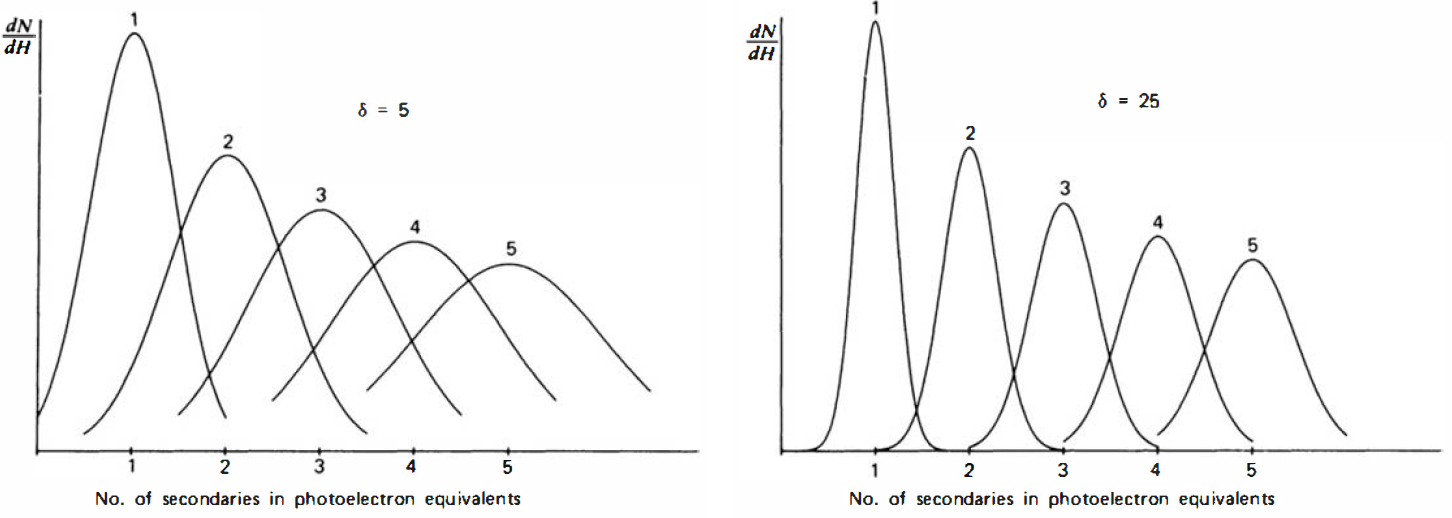
\includegraphics[width=0.9\textwidth]{immagini/distribuzione_elettroni_dinodo_delta.png}
\end{figure}
Vediamo come la distribuzione cambia a seconda del numero di elettroni che arrivano al secondo dinodo. Chiaramente, più è grande questo numero più queste fluttuazioni sembrano essere grandi cioè queste distribuzioni sono larghe, ma in termini relativi le fluttuazioni statistiche diminuiscono. Il motivo è che la dispersione relativa è definita come $(\sigma/\mu)^2$ dove $\sigma$ è la deviazione standard e $\mu$ la media, quindi nel caso della distribuzione di Poisson è uguale a $1/\delta$. Ne segue che le fluttuazioni statistiche in termini relativi diminuiscono quando consideriamo un'emissione maggiore, quindi un $\delta$ più grande. Ciò ha una sua importanza, perché tanto più è elevato il segnale che si produce all'anodo, tanto più è probabile che questo si possa distinguere da un eventuale segnale di rumore dovuto ad esempio a questioni termiche, le quali danno luogo ad un segnale che tipicamente è molto frequente ma ha un'ampiezza piccola, in quanto viene emesso da un elettrone che dà luogo a questa catena. 

\subsection{Configurazione dinodi}
La geometria dei dinodi, cioè il modo in cui vengono disposti, è fondamentale, perché come abbiamo detto questi elettroni devono essere guidati da un dinodo all'altro. Ci sono tantissime configurazioni che sono state studiate nell'arco della storia, in particolare quelle più utilizzate sono di quattro tipi:
\begin{figure}[H]
   \centering
   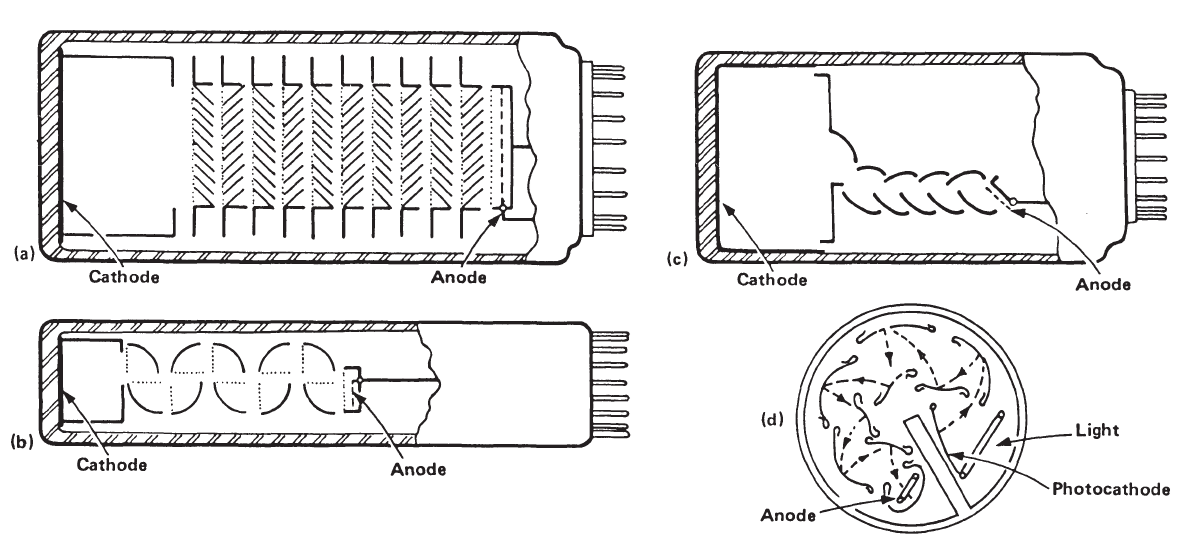
\includegraphics[width=0.9\textwidth]{immagini/geometrie_dinodi.png}
\end{figure}
Le configurazioni sono in ordine
\begin{enumerate}[label=(\alph*)]
   \item a veneziana;
   \item a box e a griglia;
   \item focalizzati linearmente;
   \item focalizzati circolarmente.
\end{enumerate}
Quella che abbiamo visto fino ad ora è di tipo $\rm (c)$, cioè focalizzati linearmente.

Andiamo a guardare quali sono le deviazioni dalla linearità in base alla configurazione scelta:
\begin{figure}[H]
   \centering
   \includegraphics[width=0.65\textwidth]{immagini/deviazioni_linearità.png}
\end{figure}
Abbiamo detto che ci aspettiamo che questo segnale mantenga una certa proporzionalità rispetto all'energia che viene depositata, ma in realtà questo non è sempre vero: a volte se il flusso di elettroni è molto elevato si può perdere la linearità, quindi finché la curva di deviazione dalla linearità si mantiene uguale a zero stiamo lavorando in un ottimo regime di lavoro. Possiamo evincere dal grafico come la configurazione con i fotomoltiplicatori focalizzati linearmente sia quella migliore, in quanto ha un'ampia regione di lavoro dei valori di corrente in cui le deviazioni dalla linearità sono dello $0\%$, mentre le altre configurazioni hanno deviazioni nulle soltanto per basse correnti, quindi per bassi numeri di elettroni che vengono prodotti e raccolti all'anodo.

\subsection{Alimentazione}
Per quanto riguarda l'alimentazione, si applica un'alta tensione al fotomoltiplicatore avente valori di $600-700 \rm \; V$, la quale viene poi suddivisa tra i diversi dinodi utilizzando dei partitori di tensione.
\begin{figure}[H]
   \centering
   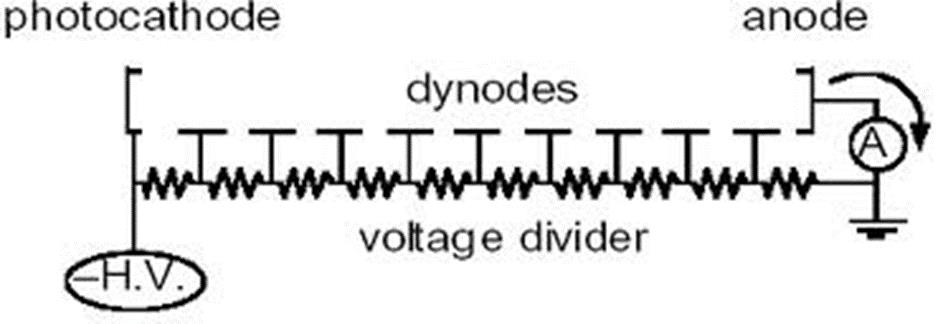
\includegraphics[width=0.65\textwidth]{immagini/partitore_tensione.png}
\end{figure}
In genere tra fotocatodo e primo dinodo è applicata una tensione maggiore, allo scopo di focalizzare meglio gli elettroni emessi dal fotocatodo.

Ci sono due modalità di lavoro: o si lavora con un fotocatodo a potenziale negativo e l'anodo a zero oppure viceversa si pone il fotocatodo a zero e l'anodo a una tensione positiva (in figura è riportata soltanto la prima di queste due configurazioni). Questi due diversi modi di lavorare sono equivalenti poiché ciò che conta è la differenza di potenziale, in quanto si deve passare da un potenziale più basso ad un potenziale più alto.
\subsection{Guadagno vs tensione}
La tensione di alimentazione del fotomoltiplicatore ha un'influenza sul segnale finale. Infatti il fattore $\delta$ può cambiare a seconda della tensione di lavoro: più questa è alta, più gli elettroni verranno accelerati tra un dinodo e l'altro raggiungendo quindi energie più alte, dunque sarà maggiore il numero di elettroni emessi e di conseguenza il numero di elettroni che riescono a raggiungere il dinodo successivo.

Se indichiamo con $V_d$ la differenza di potenziale tra due dinodi consecutivi, $\delta$ sarà dato da
\begin{equation*}
   \delta=K V_d
\end{equation*}
dove $K$ è una costante di proporzionalità. Possiamo allora riscrivere il guadagno come
\begin{equation*}
   G=\alpha \delta^n
   =\alpha \bigl( KV_d \bigr)^n
\end{equation*}
dove $n$ è il numero di dinodi. In definitiva il guadagno dipende dalla tensione tramite una legge di potenza, da cui segue che basta anche una leggera variazione nella tensione di lavoro per avere una variazione nel guadagno notevole. Ecco perché gli alimentatori che si adoperano per alimentare i fotomoltiplicatori devono essere degli alimentatori abbastanza stabili, che mantengono il valore di tensione il più stabile possibile.

\vspace{0.2cm}Cerchiamo adesso di capire quanto varia il guadagno quando variamo la tensione di 1 V. Questa variazione, che normalmente si esprime in termini percentuali, prende il nome di coefficiente di guadagno ed è qualcosa che misuriamo in laboratorio. Infatti misurare il guadagno del fotomoltiplicatore non è un'operazione facile, perché per misurarlo dovremmo lavorare in condizioni di singolo fotoelettrone, quindi dovremmo metterci nelle condizioni di far produrre al fotocatodo un solo elettrone e vedere cosa si ottiene all'anodo, la quale non è un'operazione semplice. Ciò che invece possiamo fare è studiare l'andamento del guadagno in funzione della tensione e quindi valutare queste variazioni percentuali del guadagno al variare della tensione. Questa seconda operazione è quella che svolgiamo in laboratorio, ossia effettuiamo delle misure con un fotomoltiplicatore aumentando di volta in volta la tensione, esplorando un certo intervallo di tensioni e andando a cercare di capire quanto cambia il segnale in uscita. Infatti aumentando la tensione aumenta il guadagno, quindi aumenta il numero di elettroni che arrivano all'anodo e pertanto il segnale aumenterà in ampiezza, quindi possiamo studiare di quanto aumenta o diminuisce il segnale quando cambiamo la tensione di un certo valore. Possiamo allora studiare la derivata dell'ampiezza del segnale in funzione della tensione e valutare il coefficiente di guadagno, che sarà dato dalla rivelazione
\begin{equation*}
   \frac{1}{G}\dv{G}{V}
\end{equation*}
e che viene espresso in \%/V.\footnote{Tutta questa parte è poco chiara ma non ho trovato nulla che c'entrasse sui libri.}

\subsection{Risposta temporale}
Tipicamente gli elettroni vengono emessi con tempi molto rapidi, minori del decimo di nanosecondo. Tuttavia il fattore preponderante nella produzione del segnale in termini temporali è il tempo che impiegano questi elettroni per passare dal catodo fino all'anodo. Questo è un tempo dell'ordine delle decine di nanosecondi, dunque non è trascurabile.

Se questo tempo fosse fisso, cioè se fosse sempre lo stesso ogni volta che viene emesso un elettrone dal catodo, non avremmo alcun problema in quanto costituirebbe un ritardo noto presente ogni qualvolta si effettua una misura di timing. Tuttavia, per diverse ragioni esiste una dispersione di questo tempo di transito (detto transit time) che prende il nome di TTS (Transit Time Spread). Tali fluttuazioni possono essere anche dell'ordine di alcuni nanosecondi, e ciò limita l'utilizzo del fotomoltiplicatore per applicazioni di timing spinto, dove vogliamo risoluzioni temporali particolarmente ottimali, dell'ordine del nanosecondo o anche inferiori. Alcuni fotomoltiplicatori migliorano questo aspetto con un'opportuna geometria dei dinodi oppure diminuendo il numero di fotoelettroni, quindi lavorando in condizione di illuminazione del fotomoltiplicatore un po' più basse, però non sempre è possibile.

\subsection{Schermo magnetico}

I fotomoltiplicatori lavorano con elettroni di pochi elettronVolt, quindi sono elettroni molto poco energetici che possono subire delle deviazioni anche a seguito della presenza del campo magnetico terrestre. Ecco perché i fotomoltiplicatori, a seconda di come vengono orientati, in linea di principio potrebbero funzionare in maniera leggermente diversa, perché potrebbero avere un orientamento rispetto al campo magnetico terrestre diverso a seconda di come viene posizionato il fotomoltiplicatore.

Per evitare questi problemi, quello che si fa è circondare il fototubo con un materiale che è in grado di schermare questi campi magnetici non eccessivamente elevati come ad esempio quello terrestre. Questi materiali prendono il nome di mu-metal: essi sono delle leghe metalliche ad alta permeabilità magnetica, quindi formano un vero e proprio schermo per i campi magnetici, in maniera tale che gli elettroni che vengono prodotti all'interno non subiscano effetti di deviazione dovuti a questi campi magnetici così poco intensi.

Certe volte tuttavia si ha l'esigenza di posizionare i fotomoltiplicatori all'interno dei campi magnetici di valore più elevato perché magari si vuole misurare l'impulso di una particella deviando il percorso di questa tramite campi magnetici che possono essere anche molto più intensi rispetto a quelli tipicamente derivanti da fonti naturali. In questo caso i fotomoltiplicatori non possono essere adoperati, per cui quello che si fa è trovare dei degni sostituti del fotomoltiplicatore che vedremo a breve e che possono lavorare anche in presenza di campi magnetici.

\subsection{Il rumore (noise)}
Un aspetto importante riguarda il noise, cioè il rumore. Come abbiamo già visto, la principale fonte di rumore in un fotomoltiplicatore è l'emissione termoionica di elettroni da parte del fotocatodo, ma anche da parte di altri materiali che costituiscono il fotomoltiplicatore. Tipicamente viene emesso un solo fotoelettrone alla volta, per cui il segnale spurio (cioè dovuto a rumore) che si produce è di bassa ampiezza, dunque è importante avere dei segnali fisici più elevati in maniera tale da poterli discriminare dal rumore.

Il rumore può essere diminuito abbassando la temperatura, sebbene ciò non si faccia quasi mai.

Un altro aspetto importante sempre in termini di rumore è quello di evitare di esporre il fotomoltiplicatore alla luce anche quando non si sta lavorando col fotomoltiplicatore, quindi persino quando trasportiamo un fotomoltiplicatore da un luogo ad un altro dobbiamo avere l'accortezza di evitare l'esposizione alla luce. Il motivo è che i materiali vetrosi che vengono adoperati soprattutto nel catodo possono emettere luce di fosforescenza anche per tempi molto lunghi dell'ordine delle ore, quindi se per caso il fotomoltiplicatore viene esposto alla luce bisogna poi attendere un tempo che può essere anche dell'ordine delle ore prima di poterlo adoperare nuovamente, altrimenti potremmo avere effetti indesiderati dovuti a questi fenomeni di fosforescenza del vetro. 

Altre fonti di rumore in un fotomoltiplicatore possono essere:

\begin{itemize}[leftmargin=0.5cm]
   \item La radioattività del vetro, in quanto nel vetro possono essere presenti degli isotopi radioattivi come il potassio-40 $\rm ^{40}K$ o il torio Th che emettono radiazione che viene amplificata nel fotomoltiplicatore;
   \item La radiazione cosmica che incide non solo sul rivelatore ma anche all'interno del tubo;
   \item Correnti di fuga nei supporti degli elettrodi, per cui ci vuole particolare cura nel cercare di isolare gli elettrodi presenti in un fotomoltiplicatore.
\end{itemize}

Un altro aspetto che potrebbe verificarsi sono i cosiddetti afterpulses, impulsi che avvengono dopo il segnale principale i quali possono avere delle conseguenze importanti soprattutto nelle misure di timing, perché tali misure prevedono un start e uno stop quindi se per caso ci sono degli impulsi spuri lo start e lo stop potrebbero non essere quelli effettivamente desiderati. Chiaramente anch'essi costituiscono una fonte di rumore.

Possiamo vedere gli afterpulses nel seguente grafico, dove è riportato un tipico segnale di un fotomoltiplicatore visto all'oscilloscopio, quindi sulle ascisse sono riportati i tempi e sulle ordinate i valori di tensione:
\begin{figure}[H]
   \centering
   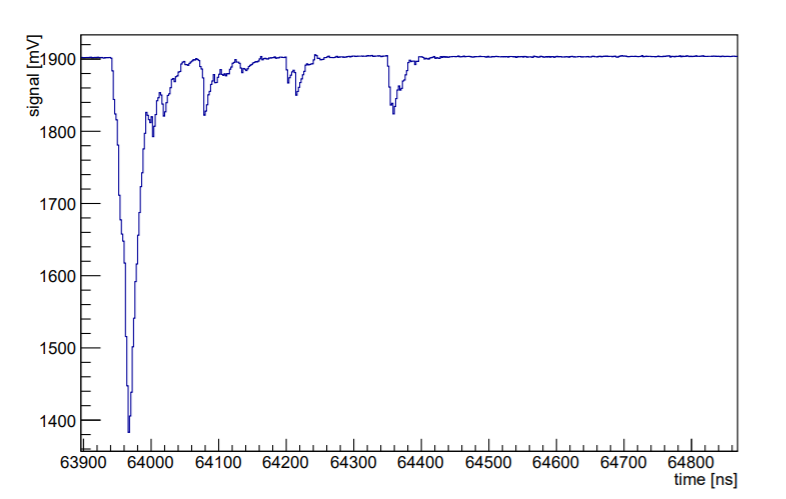
\includegraphics[width=0.7\textwidth]{immagini/afterpulses.png}
\end{figure}
Abbiamo un segnale molto veloce, con un tempo di discesa molto rapido dell'ordine di pochi nanosecondi per poi risalire. Dopo che è risalito notiamo la presenza di piccoli impulsi di bassa ampiezza: questi sono gli afterpulses.

Gli afterpulses possono avere diverse origini: essi possono provenire da
\begin{itemize}[leftmargin=0.5cm]
   \item reazioni luminose: i dinodi colpiti dagli elettroni possono emettere fotoni che, se arrivano al fotocatodo, danno origine ad un effetto fotoelettrico e quindi ad afterpulses, che sono ovviamente ritardati rispetto all'impulso principale perché dobbiamo considerare il tempo che impiega la luce a tornare indietro verso il fotocatodo. Ritardi tipici in questo caso sono dell'ordine di $20-100$ ns;
   \item ionizzazione di gas residui nel fototubo: infatti il fototubo, cioè il tubo in cui sono inseriti i dinodi, lavora in condizioni di vuoto, però per quanto il vuoto realizzato all'interno del fototubo possa essere spinto sono sempre presenti degli atomi di gas residuo, per cui può succedere che gli elettroni ionizzino questo gas residuo e gli ioni positivi migrino verso il fotocatodo (perché questo si trova a un potenziale negativo) liberando elettroni, producendo quindi dei segnali ritardati con ritardi tipici di 100 nanosecondi o anche microsecondi, perché questo impulso viene prodotto da uno ione che ha dovuto viaggiare verso il fotocatodo, il quale ha una mobilità ridotta rispetto a quella degli elettroni.
   \item backscattering degli elettroni: durante il processo di amplificazione, alcuni elettroni possono essere rimandati indietro dall'urto, ritornando al primo dinodo e generando un altro segnale ritardato rispetto al primo.
\end{itemize}

\subsection{Forma e dimensioni}
Ci sono diverse possibilità per le dimensioni e la forma di un fotomoltiplicatore. Tipicamente sono oggetti ingombranti e di solito hanno una forma tubolare, ma potrebbero avere anche forme un po più particolari come quelli adoperati nell'esperimento KM3NeT per la rivelazione dei neutrini, i quali hanno grande area perché cercano di captare un quantitativo di luce che sia il più grande possibile in quanto la luce prodotta in mare dall'interazione dei neutrini (quindi dei muoni) è abbastanza bassa, dunque bisogna raccogliere il più possibile la luce prodotta.

\comment{
\subsection{Applicazioni}Ci sono tantissime applicazioni dei fotomoltiplicatori non solo nel campo della della fisica ma anche in medicina e biologia ad esempio una delle applicazioni più note di fotomoltiplicatori nel campo della fisica riguarda l'esperimento supercambio cande non so se ne abbiamo parlato non abbiamo parlato non abbiamo affrontato ancora neutrini niente non abbiamo parlato di neutrini va bene comunque questo è un grosso rivelatore che è stato realizzato all'interno di una miniera abbandonata questa miniera è stata riempita di acqua e le panetti sono state ricoperte vedete da questi fotomoltiplicatori di grande area e il motivo appunto che i neutrini interagendo con l'acqua possono produrre ad esempio muoni che poi emettono ovviamente della radiazione nell'attraversare l'acqua per pareffetto cerenco quindi massiva misurare questa radiazione vedete sono tanti occhi insostanzialmente questo esperimento ha lavorato per diversi anni vedete qui ad esempio una fase di intervento queste sono delle persone su un buon muone che vanno a sostituire comunque a intervenire su alcuni di questi 

fotomoltiplicatori questo esperimento diceva ha preso dati per tantissimi anni diversi anni fa c'è fu un incidente si rupperò praticamente tutti i fotomoltiplicatori attraverso una reazione a cadena cioè si si si è rotto un fotomoltiplicatore e poi sono esposito tutti gli altri comunque ormai mi sembra che non prenda più dati questo estremento oppure ad esempio nel campo del raggi cosmici raggi cosmici nell'attraversare l'attraversfera possono produrre luce di florescenza anche questa è una luce molto debole e utilizzando degli opportuni telescopi di florescenza si può convogliare attraverso un sistema di specchi la luce di florescenza verso un fotosensore che in questo caso è costituito da fotomoltiplicatori ad esempio l'esperimento ger che è il più grande esperimento per la fisica dei raggi cosmici utilizza proprio sistemi di questo tipo oppure al ser non ovviamente ci sono tantissimi rivelatori che utilizzano questo tipo di fotosensori ovviamente e qui il problema è al solito l'utilizzo di campi magnetici e in questa tabella vedete giusto per avermi idea i diversi esperimenti che fanno uso di scintillatori e di fotomoltiplicatori ovviamente sono anche grossi numeri quelli in gioco anche nel campo della ricerca dell'antimateria sulla soluzione spaziale sono installati i rivelatori come ad esempio ams che presenta il termine dei fotomoltiplicatori quindi gli impieghi sono veramente molto ampi anche nel campo della bioluminescenza quindi la rivelazione di luce messi ad organismi viventi anche questo caso siccome la luce messi è molto debole si utilizzano dei fotomoltiplicatori tuttavia 
}

\section{Avalanche PhotoDiodes (APD)}
In molte applicazioni, i fotomoltiplicatori presentano delle problematiche:
\begin{itemize}
   \item a volte hanno delle dimensioni troppo grandi rispetto all'area sensibile;
   \item sono influenzati dai campi magnetici;
   \item hanno una risposta spettrale che non sempre è adatta alla luce da rivelare;
   \item hanno un'efficienza quantica non elevata, dell' ordine del $20-30\%$;
   \item la stabilità del guadagno, cioè quanto è stabile il guadagno che abbiamo definito, non è ottimale in quanto dipende molto dalla tensione;
   \item dobbiamo adoperare delle tensioni di alimentazione elevate, di diverse centinaia di Volt fino anche al kV.
\end{itemize}
Per tutti questi motivi, nel corso degli anni sono stati sviluppati dei fotosensori più compatti basati sull'utilizzo di materiale semiconduttore, quindi sono dei fotosensori a stato solido. I primi che andremo a vedere sono i fotodiodi a valanga, di cui i primi prototipi sono stati sviluppati una quarantina d'anni fa. Questi primi prototipi avevano dimensioni molto piccole, con superfici dell'ordine del millimetro quadro; inoltre erano particolarmente sensibili all'infrarosso, quindi non si adattavano agli scintillatori che emettono nell'UV, avevano un basso guadagno e costavano molto. Sembravano quindi dei rivelatori non particolarmente performanti, ma in anni recenti sono state migliorate diverse caratteristiche di questi fotosensori, quindi adesso abbiamo degli APD che hanno superfici più estese dell'ordine di decine di millimetri quadri, hanno una sensibilità maggiore nel blu e nell'ultravioletto che è quella che ci interessa di più per la luce di scintillazione, il costo si è abbassato e hanno un guadagno relativamente elevato. Diciamo relativamente perché confrontato con il guadagno del fotomoltiplicatore, che è dell'ordine di $10^6-10^7$, quello dell'APD, proprio per il suo principio di funzionamento, è dell'ordine di $10^2$.

Infine gli APD hanno l'enorme vantaggio di lavorare con tensioni più basse rispetto a quelle dei fotomoltiplicatori. Proprio per questo motivo vengono utilizzati in diverse applicazioni dove sono presenti gli scintillatori.

\subsection{Principio di funzionamento}
L'idea alla base degli APD è quella di adoperare dei materiali semiconduttori drogati. Ciò vuol dire che sono stati introdotti alcuni atomi di un elemento diverso che possono essere elementi donori, quindi con un eccesso di elettroni rispetto a un atomo che costituisce il cristallo oppure accettori, cioè con un difetto di elettroni. A seconda del tipo di elemento che abbiamo utilizzato per drogare i semiconduttori si parla di materiali drogati di tipo p o di tipo n. Andando a realizzare delle particolari giunzioni con i semiconduttori, è possibile creare dei rivelatori di particelle, ma anche rivelatori di luce.

Tipicamente un APD ha una struttura come quella che vediamo schematizzata nelle figure seguenti:

\begin{minipage}{0.5\textwidth}
   \begin{figure}[H]
      \centering
      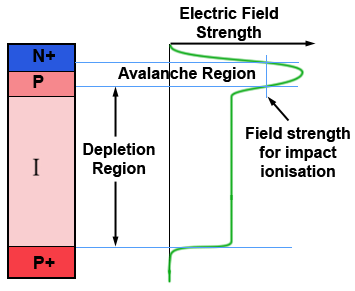
\includegraphics[width=0.9\textwidth]{immagini/APD_1.png}
   \end{figure}
\end{minipage}
\begin{minipage}{0.5\textwidth}
   \begin{figure}[H]
      \centering
      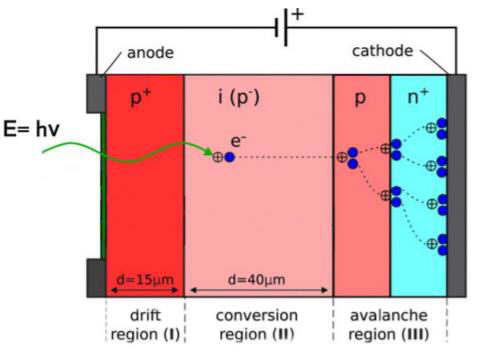
\includegraphics[width=\textwidth]{immagini/APD_2.png}
   \end{figure}
\end{minipage}

\vspace{0.4cm}In sequenza abbiamo le seguenti zone:
\begin{itemize}
   \item un primo strato drogato di tipo p;
   \item uno strato detto parte intrinseca e indicata con i, dove con intrinseco intendiamo un materiale che è stato drogato con la stessa concentrazione di donori e accettori;
   \item un altro strato drogato di tipo p;
   \item un ultimo strato drogato di tipo n.
\end{itemize}
Tale sequenza di strati fa sì che si venga a realizzare una regione ottimale per la rivelazione.

Entriamo più nel dettaglio su ciò che avviene fisicamente guardando la figura a destra: quando incide un fotone con energia $h \nu$, esso entra attraverso lo strato sottile $\rm p^{+}$ e interagisce da qualche parte all'interno della regione intrinseca, producendo una coppia elettrone-lacuna. A questo punto, grazie all'utilizzo di elettrodi viene creata una differenza di potenziale tra anodo e catodo, per cui l'elettrone viene accelerato e migra verso la regione di moltiplicazione (costituita dalle regioni p ed n), dove può dare luogo a processi di moltiplicazione a valanga, in quanto l'elettrone può arrivare ad avere un'energia sufficiente per produrre nuove coppie elettrone lacuna, con un guadagno che non supera il valore di 100, quindi a partire da un fotone incidente, dunque da un elettrone prodotto, possiamo al massimo ottenere un centinaio di elettroni raccolti nell'elettrodo finale. I segnali quindi non vengono amplificati di molto, solo quanto serve per la rivelazione di questi fotoni.

\subsection{Parametri operativi}
Andiamo a guardare alcune caratteristiche di un APD.

\begin{itemize}[leftmargin=0.5cm]
   \item Abbiamo uno strato anti-riflesso in superficie, grazie al quale abbiamo un'elevata efficienza di rivelazione perché la maggior parte dei fotoni che incide riesce effettivamente a essere rivelata;
   \item La tensione di alimentazione è di alcune centinaia di Volt, però i guadagni non sono elevatissime, dell'ordine di $50-100$;
   \item Come tutti i rivelatori a semiconduttore, purtroppo hanno una dipendenza dalla temperatura, quindi variare la temperatura di lavoro comporta delle variazioni nel segnale in uscita, avendo anche qualche \% di variazione per ogni grado di temperatura, quindi è importante lavorare ad una temperatura stabile, e ciò in generale vale per tutti i rivelatori a semiconduttore;
   \item Sono particolarmente adatti per convertire la luce proveniente o da Fibre WLS perché queste hanno sezioni piccole, o da piccoli scintillatori, in quanto è chiaro che uno scintillatore di dimensioni grandi non può essere accoppiato con un singolo APD non avendo una superficie sufficiente ad assicurare la rivelazione dei fotoni di scintillazione;
   \item Hanno delle proprietà temporali di timing abbastanza buone;
   \item Hanno dimensioni che possono arrivare anche a $5 \times 5 \; \rm mm^2$ e oltre\footnote{Per dare un'idea, hanno le dimensioni di una monetina da 5 centesimi.};
   \item Il segnale è proporzionale al numero di fotoni incidenti, quindi manteniamo l'informazione sull'energia depositata o comunque sul numero di fotoni incidenti.
\end{itemize}
%Gli APD sono stati adoperati all'interno dell'esperimento ALICE per andare a leggere la luce raccolta da fibre WLS, le quali scorrevano all'interno di un modulo che è costituito da strati alternati di piombo e scintillatore che veniva adoperato proprio per un calorimetro. In questo caso quindi la luce prodotta nello scintillatore veniva raccolta da queste fibre e le fibre venivano convogliate sulla superficie dell'APD. 

\section{Silicon PhotoMultipliers (SiPM)}
L'ultima categoria di fotosensori più recenti sono i silicon photomultipliers. Il fatto che si adoperi la parola fotomoltiplicatore nel nome ci fa capire che evidentemente qui il guadagno è più elevato, più simile a un fotomoltiplicatore. Abbiamo quindi il vantaggio di avere un guadagno elevato ma abbiamo un materiale a semiconduttore, infatti anche in questo caso abbiamo l'utilizzo di un rivelatore che è molto simile all'APD, in quanto un SiPM è costituito da una matrice di APD di piccolissime dimensioni, quindi come se fosse un rivelatore a pixel dove ogni pixel è una sorta di APD che viene adoperato in in regime limitato Geiger-Müller.
\begin{figure}[H]
   \centering
   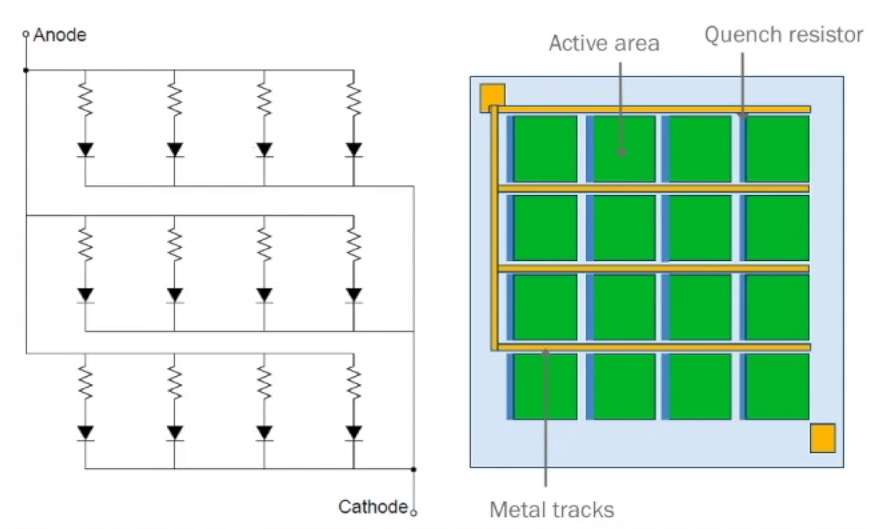
\includegraphics[width=0.8\textwidth]{immagini/SiPM.png}
\end{figure}
\subsection{Principio di funzionamento}
Vediamo come funziona. Le varie celle che vediamo hanno dimensioni che vanno dalle decine alle centinaia di micron, quindi abbiamo densità molto elevate, dell'ordine di 1000 pixel per millimetro, e tutte queste celle lavorano in parallelo. Se una di queste celle viene colpita da un fotone e quindi dà luogo a un segnale, possiamo andare a sommare tutti questi segnali tra di loro e quindi avere un segnale in uscita che è proporzionale a quante celle sono state colpite dai fotoni, dunque a quanti fotoni hanno inciso sul rivelatore. La validità di tale schema si basa sul presupposto che su ogni singola cella incida un solo fotone, perché se dovessero incidere più fotoni si perderebbe la linearità che abbiamo supposto. Siccome normalmente i SiPM hanno celle di dimensioni molto piccole, normalmente lavorano in queste condizioni di linearità. Inoltre ognuna di queste celle ha una sua resistenza di spegnimento, detta resistenza di quenching, la quale permette di riportare il SiPM verso le condizioni di lavoro ottimali\footnote{La funzione della resistenza di quenching è quella di spegnere la valanga rendendo la tensione effettiva minore della tensione di breakdown.}. Sostanzialmente il SiPM lavora come se fosse un rivelatore multiplo, quindi come tanti rivelatori che lavorano insieme, e il segnale che preleviamo alla fine è la somma dei segnali di tutte le celle.

\subsection{Vantaggi e svantaggi}
Vediamo che vantaggi ha:
\begin{itemize}[leftmargin=0.5cm]
   \item Lavora a tensione molto bassa ($30-70$ V);
   \item Ha un'efficienza quantica del $20-40\%$;
   \item Ha guadagni elevati, fino a $10^6$, il quale dipende dal numero di pixel a disposizione;
   \item Ha una risoluzione temporale molto buona ($\ll 1 \; \rm ns$);
   \item \E indipendente dal campo magnetico.
\end{itemize}
Tuttavia ancora si deve lavorare un po' sulle dimensioni le quali sono ancora piccole e sul dark count rate, cioè quel rumore che è sempre presente nei fotosensori anche in essenza di radiazione, che in questo caso può essere anche molto elevato (100 kHz 1 MHz /mm 2), dipende dal produttore.

\subsection{Analisi del segnale}
Come abbiamo detto le celle lavorano in parallelo, pertanto se guardiamo all'oscilloscopio un tipico segnale prodotto da un SiPM messo in persistenza\footnote{Mettere in persistenza un segnale significa non fare aggiornare il display dell'oscilloscopio, facendo accumulare tutti i segnali che vi arrivano nel tempo, quindi quello che è stato visualizzato non si cancella ma rimane nello schermo e il nuovo segnale viene sovrapposto a quello che abbiamo visto prima.} osserveremo una distribuzione dei segnali come quella in figura:
\begin{figure}[H]
   \centering
   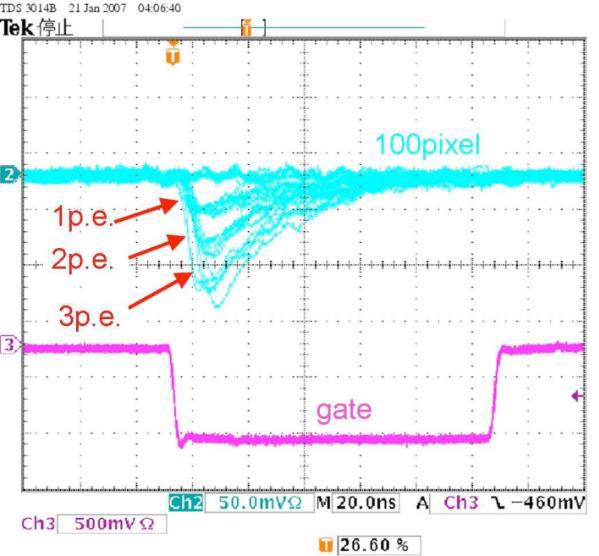
\includegraphics[width=0.6\textwidth]{immagini/segnale_persistenza_SiPM.png}
\end{figure}
Quelli che vediamo sono segnali che non hanno ampiezza qualunque, bensì hanno ampiezze quantizzate, ossia assumono dei valori discreti pari a multipli di un certo livello. I segnali che stiamo vedendo sono relativi alla rivelazione dei singoli fotoelettroni, quindi l'ampiezza del segnale è proporzionale al numero di fotoelettroni emessi, dunque al numero di celle colpite (ricordiamo che stiamo supponendo che incida un fotone per cella). Ecco perché avviene questa discretizzazione del segnale, perché ogni cella lavora come se fosse un Geiger, ossia un rivelatore on/off.

Se andiamo a realizzare uno spettro delle ampiezze di questi segnali, chiaramente troveremo una distribuzione a picchi, che corrisponde al fatto che le ampiezze non possono essere qualunque, ma assumono dei valori ben precisi:

\begin{figure}[H]
   \centering
   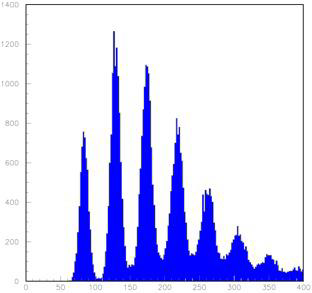
\includegraphics[width=0.6\textwidth]{immagini/spettro_SiPM.png}
\end{figure}

Avremo quindi che il primo picco è quello corrispondente al primo fotoelettrone, il secondo picco è quello corrispondente a due fotoelettroni e così via.

\subsection{Photon Detection Efficiency (PDE)}
Anche qui abbiamo una efficienza di rivelazione, detta photon detection efficiency e che dipende da diversi parametri:
\begin{enumerate}
   \item Fill factor geometrico;
   \item L'efficienza quantica, che dipende della lunghezza d'onda;
   \item La probabilità di trigger della valanga.
\end{enumerate}

\textbf{Fill factor}

Tale fattore dipende dal fatto che abbiamo una matrice, quindi l'area sensibile è soltanto la parte centrale, in quanto abbiamo inevitabilmente dei bordi che rappresentano un'area morta, quindi se il fotone dovesse incidere su questi bordi verrebbe perso. Quantitativamente tale contributo è dato dal rapporto tra l'area attiva di rivelazione e l'area complessiva, quindi più siamo in grado di realizzare bordi sottili, maggiore sarà l'efficienza dovuta al fill factor. \E altresì chiaro che, a parità di spessore, l'effetto del bordo è tanto più importante quanto più è piccola la dimensione del pixel. Ad esempio con celle delle dimensioni di $20 \; \rm \mu m$ abbiamo un fill factor intorno al 30\%, mentre con celle di $100 \; \rm \mu m$ arriva fino all'80\%.

\vspace{0.2cm}\textbf{Quantum Efficiency}

L'efficienza quantica è più elevata rispetto a quella che abbiamo visto nel caso dei fotomoltiplicatori tradizionali, potendo anche assumere valori superiori all'80\%, a seconda del tipo di sensore e dalla lunghezza d'onda che andiamo a rivelare.

\begin{figure}[H]
   \centering
   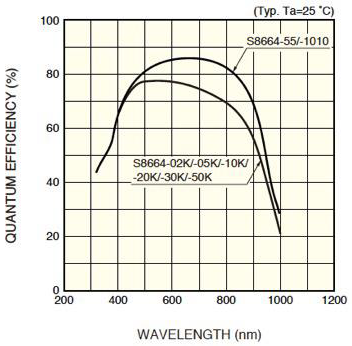
\includegraphics[width=0.6\textwidth]{immagini/Efficienza_quantica_SiPM.png}
\end{figure}

\textbf{Probabilità di trigger}

Una volta che la radiazione ha inciso e ha prodotto una coppia, quest'ultima riesce a produrre un segnale sufficientemente elevato, quindi a dare luogo a un trigger e dunque a una rivelazione?

La risposta è che la  probabilità di triggerare una valanga dipende dalla posizione in cui è stata creata la carica, dal tipo di carica (elettrone/lacuna) e dalla tensione di alimentazione.

\begin{figure}[H]
   \centering
   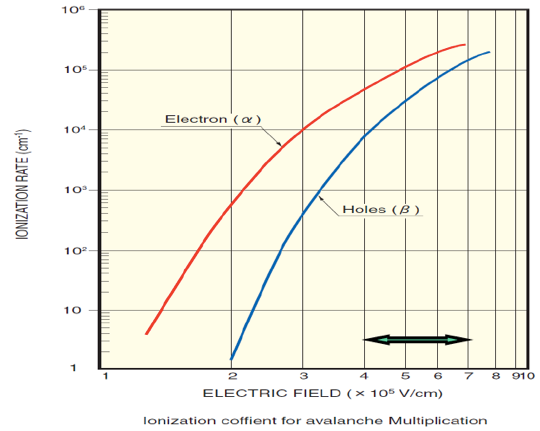
\includegraphics[width=0.65\textwidth]{immagini/probabilita_trigger_SiPM.png}
\end{figure}

In figura possiamo vedere due curve dell'andamento della probabilità (una relativa agli elettroni e l'altra alle lacune) al variare del campo elettrico applicato, quindi della tensione. Notiamo come questa cresce con la tensione applicata.

\subsection{Possibili strutture}
Ci sono diverse strutture per i SiPM, ma in generale si dividono in due tipologie: p su n o n su p, a seconda che la regione sensibile sia rispettivamente di tipo n o p.

\begin{figure}[H]
   \centering
   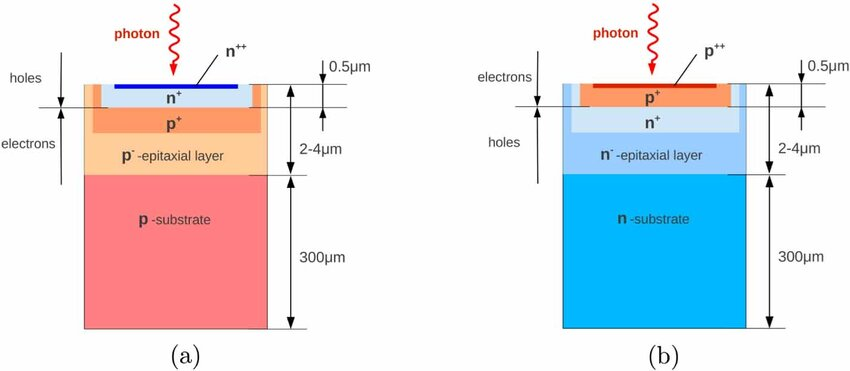
\includegraphics[width=0.9\textwidth]{immagini/strutture_SiPM.png}
   \caption*{(a): tipo p su n, (b): tipo n su p.}
\end{figure}

\subsection{Possibili applicazioni}

Avendo dimensioni molto piccole, i SiPM possono essere adoperati per la lettura delle fibre WLS. Poiché hanno un guadagno notevole, sono utili soprattutto nel caso in cui abbiamo una sola fibra e quindi ci aspettiamo poca luce.

Anche per la PET si sta pensando di sostituire il classico fotomoltiplicatore con dei SiPM.

\subsection{Confronto tra fotosensori}

Facciamo in conclusione un confronto tra i fotosensori visti:

\begin{center}
   \begin{tabular}{|c|c|c|c|}
      \hline
       & PMT & APD & SiPM\\
      \hline
      &&&\\[-0.45cm]
      Guadagno & $10^6-10^7$ & $\sim 100$ & $10^6-10^6$\\
      \hline
      &&&\\[-0.45cm]
      Tensione di lavoro (V) & $1-2 \cdot 10^3$ & $300 - 500$ & $<100$\\
      \hline
      &&&\\[-0.45cm]
      Dark count (Hz) & $<10^3$ & & $0.1-1$ M\\
      \hline
      $\begin{array}{cc}
         \text{Photon detection}\\
         \text{efficiency (blu-verde)}
      \end{array}$
      & $20-30\%$ & $75-80\%$ & $20-50\%$\\
      \hline
   \end{tabular}
\end{center}
Da un lato abbiamo il PMT che si caratterizza per avere degli ottimi guadagni ma ha una tensione di lavoro molto elevata con un dark count rate abbastanza basso e ha efficienza quantica bassa, ma in compenso ha un'area sensibile abbastanza elevata. Abbiamo poi i materiali semiconduttori ossia APD e SiPM che si caratterizzano soprattutto per le basse tensioni di lavoro, le efficienze tipicamente più elevate, guadagni che possono anche essere confrontabili con quelli del fotomoltiplicatore tradizionale ma hanno lo svantaggio di avere delle superfici abbastanza ridotte.

\section{L'occhio umano}

\textit{Questa sezione verrà completata in seguito}.

\comment{Possiamo immaginare anche il nostro occhio come un fotosensore. Dopo aver attraversato diversi strati di materiale diverso, la luce arriva a incidere sulla retina, che possiamo immaginare come se fosse un vero e proprio rivelatore costituita da delle sorta di pixel che sono i nostri fotorecettori. In particolare la retina è costituita da due tipi di fotorecettori:
\begin{itemize}[leftmargin=0.5cm]
   \item Coni: localizzati nella parte centrale, destinati alla percezione dei colori. Circa $6-7$ milioni;
   \item Bastonelli: localizzati nella zona periferica, particolarmente sensibili anche a pochi fotoni. Circa 120 milioni
\end{itemize}
coni e bastoncelli  secondo se siete interessati alla visione di urna, dei colori o alla versione notturna crepuscolare. Intervengono dei recettori, fotorecettori diversi, in particolare i coni sono destinati alla visione di urna, quindi la percezione dei colori sono un numero più ridotto rispetto ai basso in celli, tipicamente si concentrano vicino nella parte centrale della retina, vicino all'asse ottico. I basso in celli invece che sono utilizzati per la visione notturna sono molti di più e sono distribuiti un po' in tutta la regione della retina. Comunque perché faccio questo discorso? Perché potremmo cercare di capire che prestazioni ha il nostro occhio in termini di auto rivelazione. Alla fine noi abbiamo parlato di strumenti che vanno a percepire della luce che il nostro occhio è lì in principio e non è in grado di percepire, o comunque non è facile percepirli. Allora in totale posso immaginare di avere un occhio standard all'incirca 100 milioni di fotorecettori, quindi equivale al dire 100 megapixel se dovessimo adoperare un termine simile a quello che doveriamo nel campo della rivelazione e in una singola immagine vengono interessati simultaneamente all'incirca 7 megapixel. Tuttavia l'occhio vede continuamente in modo ciclico anche 100 volte al secondo e questo ne aumenta la risoluzione. Quindi alla fine potremmo dire che complessivamente il nostro occhio può essere approssimo all'autofotosensore con 570 megapixel, quindi immaginate ovviamente delle prestazioni notevoli. Chiaramente la sua risposta dipenderà dalla lunghezza d'onda della luce che incide, in particolare di nostro occhio ottimizzato per vedere le lunghezze d'onda intorno al verde e giallo che appunto corrispondono anche col massimo di emissione della nostra stella nel sole, quindi non è un caso ovviamente che noi abbiamo una maggiore risposta proprio in corrispondenza di queste lunghezze d'onda. Concludo facendovi vedere questo articolo che uscito qualche anno fa a Sonnecer, è stato appunto una notizia particolare, io insegnavo a Topp, fin l'anno scorso e quindi mi interessavo anche di questi aspetti, sostanzialmente è stato condotto uno studio per cercare di capire se l'occhio umano fosse in grado di rivelare di riperrare i singoli fotoni, cosa che noi normalmente facciamo appunto con della strumentazione anche molto costoso e complessa, ma in realtà è stato dimostrato sperimentalmente che l'occhio umano è in grado di misurare i singoli fotoni, è stato fatto appunto uno studio sperimentale sotto determinate condizioni e si è arrivato questo risultato che ha meritato la pubblicazione su Nexar, non so se conoscete vostre riviste, penso di sì, quindi sapete che non è rivista di assoluto prestigio e questo è contestato il riassunto di questo risultato sperimentale.
}